\documentclass{article}
\usepackage[utf8]{inputenc}
\usepackage{amsmath}
\usepackage{mathtools}
\usepackage[a4paper,left=0.8in,right=0.8in,bottom=1in]{geometry}
\setlength{\parskip}{1em}
\setlength{\parindent}{2em}
\usepackage{floatrow}
\usepackage{graphicx}
\title{CS215 Assignment 1}
\author{Aquib Nawaz(190050023),Rajesh Dasari(190050030),\\Paavan Kumar(190050051)}
\date{2 September 2020}

\begin{document}

\maketitle

\section* {Question 1}
\subsection* {a)}
    The probability of each person picking their own book is given by \\
    \par
    $P(event)=\frac{N(event)}{N(SampleSpace)}$
    \par
    $N(SampleSpace)=n* (n-1)\times (n-2) ..... \times 1 = n!$\\\label{N(s)}
    The event that each person picks their own book can occur only when each person picks his own book
    \par
    $N(event)=1$
    \par
    \textbf{$P(event)=\frac{1}{n!}$}
\subsection* {b)}
    When the first m persons pick up a book,there are $n-m$ books remaining,which can be distributed among remaining $n-m$ people in exactly $(n-m)!$
    \par
    $N(event)=(n-m)!$
    \par
    $P(event)=\frac{N(event)}{N(SampleSpace)}$
    \par
    \textbf{$P(event)=\frac{(n-m)!}{n!}$\ref{N(s)}}
\subsection* {c)}
     When the first m persons pick up a book from the books of last m persons,(which can be done in exactly in $m!$ ways),there are $n-m$ books remaining with $n-m$ to chose from, which can be done in $(n-m)!$.
     \par
     $N(event)=m!(n-m)!$
     \par
     $P(event)=\frac{N(event)}{N(SampleSpace)}$
     \par
     \textbf{$P(event)=\frac{m!(n-m)!}{n!}$}
\subsection* {d)}
    The probability of a book remaining clean is $1-p$, since being clean and unclean are mutually exclusive.\\
    Since the picking of a book by a person are independent events,\\
    The remaining $n-m$ people can choose any book ,whether unclean or clean.
    \par
    $Probability=P(p_1)\times P(p_2)\times ......\times P(p_{m})\\$
    where $P(p_{i})$ is the probability of $i$th person picking a clean book, which is $1-p$
    \par
    $Probability=(1-p)^m$
\subsection*{e)}
    The probability of a book remaining clean is $1-p$, since being clean and unclean are mutually exclusive.\\
    Since exactly m people must pick clean books,the remaining $n-m$ must pick unclean books,
    \par
    $probability=P(p_1)\times P(p_2)\times .....\times P(p_{m})\times (1-P(p_{m}))\times .....\times (1-P(p_{n}))\\$
    where $P(p_{i})$ is the probability of $i$th person picking a clean book,which is $1-p$
    \par
    $probability=(1-p)^m\times p^{n-m}$
\section* {Question 2}
    By defintion ,the Standard Deviation $\sigma$, is given by 
    \par
    $\sigma^2=\frac{1}{n-1} \times \sum_{i=1}^{n} (x_i-\mu)^2 $
    \par
    $(n-1)\times \sigma^2=\sum_{i=1}^{n} (x_i-\mu)^2 \\$
    Since all $x_i$ are distinct numbers,\\ 
    No more than one of $(x_i-\mu)^2$ is zero.\\
    if $x_j-\mu=0 $,then $x_k-\mu \neq 0 \ \forall \ k \neq j$
    \par 
    $(n-1)\times \sigma^2 \geq (x_i-\mu)^2 $ ,for some $i \in {1,2....,n}\\$
    Taking square root on both sides,we get
    \par 
    $\sigma \times \sqrt{n-1} \geq |(x_i-\mu)|\\$
    Therefore,
    \par 
    $|(x_i-\mu)| \leq \sigma \times \sqrt{n-1}\\$
    \newline
    Comparing this with \textbf{Chebyshev's inequality},\\
    The number of elements such that $|x-\mu|\leq k \sigma$ is $\geq \frac{N}{k^2}$\\
    letting k = $\sqrt{N-1}$,we get\\
    we get the number to be $\frac{N}{N-1}$ which evaluates to be more than one,
    that means the inequality is always true\\
    Hence from Chebyshev's inequality, the above inequality can be esaily proved.
    
\newpage
\section*{Question 3}
    Consider the set $S_1={x_i|x_i<\tau}$ and the set $S_2={x_i|x_i>\tau}\\$
    \newline
    \textbf{Case 1}\\
    Suppose $\mu > \tau$,\\
    Then for all $x_i \in S_1$,$\mu-x_i \geq \mu-\tau$\\
    Hence by the one-sided Chebyshev's inequality,
    \par
    $\frac{N(S_1)}{N} \leq \frac{1}{1+k^2}$, where $k$ in this situation is $\frac{\mu-\tau}{\sigma}$\\
    \newline
    Using $N(S_1)=\frac{N}{2}$,by the fact that n is \textbf{even}
    \par 
    $\frac{1}{1+k^2} \geq \frac{1}{2}$
    \par 
    $1+k^2 \leq 2$
    \par
    $k^2 \leq 1 \implies |k| \leq 1$
    \par
    $\frac{\mu-\tau}{\sigma} \leq 1 \implies \mu-\tau \leq \sigma \\$
    \newline 
    \textbf{Case 2}\\
    Suppose $\mu < \tau$,\\
    Then for all $x_i \in S_2$,$x_i-\mu \geq \tau-\mu$\\
    Hence by the one-sided Chebyshev's inequality,
    \par
    $\frac{N(S_2)}{N} \leq \frac{1}{1+k^2}$, where $k$ in this situation is $\frac{\tau-\mu}{\sigma}$\\
    \newline
    Using $N(S_2)=\frac{N}{2}$,by the fact that n is \textbf{even}
    \par 
    $\frac{1}{1+k^2} \geq \frac{1}{2}$
    \par 
    $1+k^2 \leq 2$
    \par
    $k^2 \leq 1 \implies |k| \leq 1$
    \par
    $\frac{\tau-\mu}{\sigma} \leq 1 \implies \tau-\mu \leq \sigma$
    \newline
    \newline
    Combining both cases ,we get $|\mu-\tau| \leq \sigma$\\
    Hence proved
\section*{Question 4}
    The probability $P(red)=0.01$,and $P(blue)=0.99$\\
    The probability $P(seenred|red)=P(seenred and red)\times P(red)=0.99\times 0.01= 0.0099$\\
    The probability $P(seenred|blue)=P(seenred and blue)\times P(blue)=0.02\times 0.99=0.0198$\\
    The probaility $P(red|seenred)$\\
    $P(red|seenred)=\frac{P(seenred|red)}{P(seenred|red)+P(seenred|blue)}$----using bayers theorem\par
    $P(red|seenred)=\frac{0.0099}{0.0099+0.0198}$\par 
    $P(red|seenred)=\frac{1}{3}$\\
    Hence the argument will of the lawyer will be the probability that XYZ has seen it to be \texttt{red} is only \textbf{33 percent} whereas for it to be \texttt{blue} is \textbf{66 percent}.
\section*{Question 5}   
\subsection*{a)}
    $P(C_i|Z_1)=\frac{P(C_i \cap Z_1)}{P(Z_1}\\$
    Given that $P(Z_1)=1/3$ and $P(C_i \cap Z_1)=P(C_i)\times P(Z_1)$,since they are independent events.
    \par 
    $P(C_i|Z_1)=\frac{P(C_i \cap Z_1)}{P(Z_1}=\frac{1/9}{1/3}$
    \par 
    $P(C_i|Z_1)=\frac{1}{3}$
\subsection*{b)}
    Given that $Z_1$ and $C_1$ occurs,\\
    the probability of host choosing door 3 , event $H_3$  is $\frac{1}{2}$ is since both the doors contains stone,so it is equally likely for the host to choose door 2 or 3.\par 
    Hence ,$P(H_3|C_1,Z_1)=\frac{1}{2}$\\
    Given that $Z_1$ and $C_2$ occurs,\\
    the probability of host choosing door 3 , event $H_3$  is 1 is since both the door 3 contains stone and door no 1 is not to be chosen by the host.\par
    Hence ,$P(H_3|C_2,Z_1)=1$\\
    Given that $Z_1$ and $C_3$ occurs,\\
    the probability of host choosing door 3 , event $H_3$  is 0 is since both the door 3 contains car, which is not to be chosen by the host.\par
    Hence ,$P(H_3|C_3,Z_1)=0$\\
\subsection*{c)}
    We know that
    \par 
    $P(C_2|H_3,Z_1)=\frac{P(H_3|C_2,Z_1)\times P(C_2,Z_1)}{P(H_3,Z_1)}$
    \par 
    $P(C_2,Z_1)=P(C_2)\times P(Z_1)=\frac{1}{3}\times \frac{1}{3}= \frac{1}{9}$
    since, these are independent events
    \par 
    $P(H_3,Z_1)=P(Z_1)\times P(H_3|Z_1)$
    \par 
    $P(H_3|Z_1)+P(H_2|Z_1)=1 \implies 2\times P(H_3|Z_1)=1$---door 2 and 3 are equally probabale
    \par 
    $P(H_3|Z_1)=\frac{1}{2}$
    \par
    $P(H_3,Z_1)=P(Z_1)\times P(H_3|Z_1)=\frac{1}{3}\times \frac{1}{2} =\frac{1}{6}$
    \par
    $P(C_2|H_3,Z_1)=\frac{P(H_3|C_2,Z_1)\times P(C_2,Z_1)}{P(H_3,Z_1)}$
    \par 
    $P(C_2|H_3,Z_1)=\frac{1\times\frac{1}{9}}{\frac{1}{6}}$
    \par 
    $P(C_2|H_3,Z_1)=\frac{1}{3}$
\subsection*{d)}
    We Know that
    \par 
    $P(C_1|H_3,Z_1)=\frac{P(H_3|C_1,Z_1)\times P(C_1,Z_1)}{P(H_3,Z_1)}$
    \par 
    $P(C_1,Z_1)=P(C_1)\times P(Z_1)=\frac{1}{3}\times \frac{1}{3}= \frac{1}{9}$
    since, these are independent events
    \par 
    $P(H_3,Z_1)=P(Z_1)\times P(H_3|Z_1)$
    \par 
    $P(H_3|Z_1)+P(H_2|Z_1)=1 \implies 2\times P(H_3|Z_1)=1$---door 2 and 3 are equally probabale
    \par 
    $P(H_3|Z_1)=\frac{1}{2}$
    \par
    $P(H_3,Z_1)=P(Z_1)\times P(H_3|Z_1)=\frac{1}{3}\times \frac{1}{2} =\frac{1}{6}$
    \par
    $P(C_1|H_3,Z_1)=\frac{P(H_3|C_1,Z_1)\times P(C_1,Z_1)}{P(H_3,Z_1)}$
    \par 
    $P(C_1|H_3,Z_1)=\frac{\frac{1}{2}\times\frac{1}{9}}{\frac{1}{6}}$
    \par 
    $P(C_1|H_3,Z_1)=\frac{1}{3}$
\subsection*{e)}
    Switching is indeed \textbf{beneficial} due to probability being $\frac{2}{3}$ as compared to $\frac{1}{3}$
\subsection*{f)}
    Since the host is not intelligent,\\
    Given that $Z_1$ and $C_2$ occurs,\\
    the probability of host choosing door 3 , event $H_3$  is $\frac{1}{2}2$ since for the host it doesnt matter because he opens one of the door maybe 2 or 3\par
    Hence ,$P(H_3|C_2,Z_1)=\frac{1}{2}$\par 
    $P(C_2,Z_1)=P(C_2)\times P(Z_1)=\frac{1}{3}\times \frac{1}{3}= \frac{1}{9}$
    since, these are independent events
    \par 
    $P(H_3,Z_1)=P(Z_1)\times P(H_3|Z_1)$
    \par 
    $P(H_3|Z_1)+P(H_2|Z_1)=1 \implies 2\times P(H_3|Z_1)=1$---door 2 and 3 are equally probabale
    \par 
    $P(H_3|Z_1)=\frac{1}{2}$
    \par
    $P(H_3,Z_1)=P(Z_1)\times P(H_3|Z_1)=\frac{1}{3}\times \frac{1}{2} =\frac{1}{6}$
    \par
    $P(C_2|H_3,Z_1)=\frac{P(H_3|C_2,Z_1)\times P(C_2,Z_1)}{P(H_3,Z_1)}$
    \par 
    $P(C_2|H_3,Z_1)=\frac{\frac{1}{2}\times\frac{1}{9}}{\frac{1}{6}}$
    \par 
    $P(C_2|H_3,Z_1)=\frac{1}{3}$
    \\
    Hence ,in this case it is \textbf{not} beneficial for the contestant to change choices
\newpage
\section*{Question 6}
\begin{figure}[H]
    \ffigbox{\caption {Using the value of f = 30 percent of values}}
    {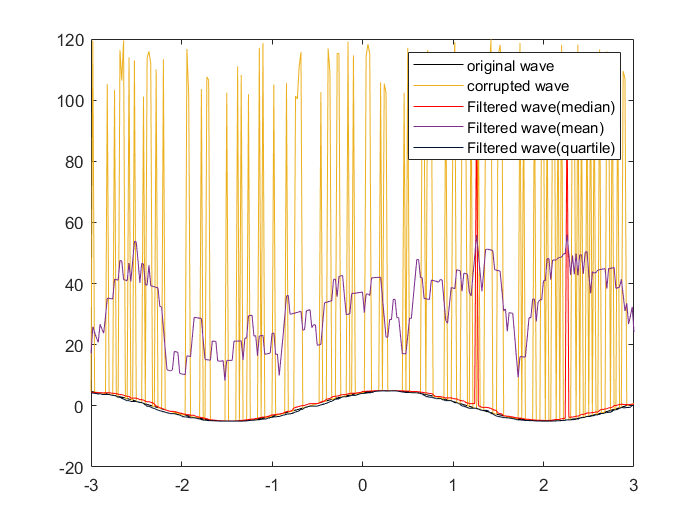
\includegraphics[width =19cm, height=14cm]{30per.png}}
\end{figure}
    For the above figure the value of \\
    \par 
    relative mean squared error for moving median filtering is 6.0307.
    \par 
    relative mean squared error for moving mean filtering is 104.2748.
    \par 
    relative mean squared error for moving mean filtering is 0.0122.
    \newline
    \par 
    \par 
    Hence,\textbf{moving quartile filtering} produced better relative mean squared error.\\
    The quartile filtering has produced the least relative mean squared error due to the fact that it contains values closer to that of the sine wave than that caused due to mean filtering and median filtering.
\begin{figure}[H]
    \ffigbox{\caption {Using the value of f = 60 percent of values}}
    {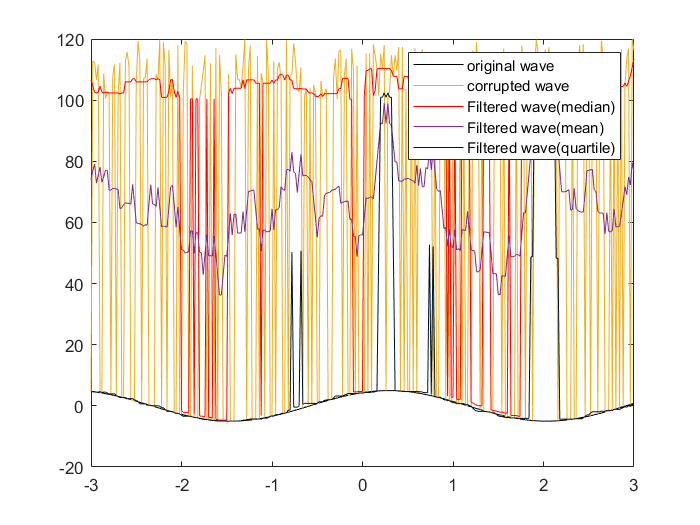
\includegraphics[width =19cm, height=14cm]{60per.png}}
\end{figure}
    For the above figure the value of \\
    \par 
    relative mean squared error for moving median filtering is 757.6717.
    \par 
    relative mean squared error for moving mean filtering is 382.3716.
    \par 
    relative mean squared error for moving mean filtering is 65.0378.
    \newline
    Hence,\textbf{moving quartile filtering} produced better relative mean squared error.\\
\subsection*{Instructions for running code}
    The code for this question is attached with the name \textbf{q6.m}.\\
    \textbf{Input format}---value of fraction\\
    \textbf{Output format}--relative mean squared error for moving median filtering\\
    ------------------------relative mean squared error for moving mean filtering\\
    ------------------------relative mean squared error for moving quartile filtering
\newpage
\section*{Question 7}
    The newMean $\mu'$ is equal to $\frac{\sum_1^{n+1} x_i}{n+1}$ and
    The oldmean $\mu$ is equal to $\frac{\sum_1^{n} x_i}{n} $
    \par 
    ${n+1} \times \mu' = \sum_1^{n+1} x_i$
    \par 
    $n \times \mu = \sum_1^{n} x_i$
    Substituting the above equation gives,
    \par 
    ${n+1} \times \mu' = n \times \mu + x_{n+1}$
    \par 
    $\mu' = \frac{n\times\mu+x_{n+1}}{n+1}$\\
    \newline
    ---------------------------------------------------------------------
    \newline
    Assuming the given array is in sorted order\\
    let the newMedian be $\tau'$ and oldMedian be $\tau$\\
    Suppose $n$ is even,then $n+1$ is odd\par 
    $\tau = \frac{x_{n/2}+x_{n/2+1}}{2}$\newline
    If $x_{n+1} > \tau$,then $\tau' = x_{n/2+1}$\\
    else $\tau' = x_{n/2}$\\
    If $n$ is odd ,then $n+1$ is even\par 
    $\tau = x_{\frac{n+1}{2}}$\newline 
    If $x_n+1 > \tau$,then $\tau' = \frac{\tau+x_{\frac{n+3}{2}}}{2}$\\
    else $\tau' = \frac{\tau+x_{\frac{n-1}{2}}}{2}$
    \newline
    ---------------------------------------------------------------------
    \newline
    let The NewStd be $\sigma'$ and OldStd be $\sigma$ 
    \par 
    $\sigma'^2 \times n = \sum_1^{n+1} {(x_i-\mu')}^2$ and $\sigma^2 \times {n-1} = \sum_1^{n} {(x_i-\mu)}^2$
    \newline 
    For any $i$,
    \par
    ${(x_i-\mu')}^2={(x_i-\mu+\mu-\mu')}^2={(x_i-\mu)}^2+2\times{(\mu-\mu')}\times{(x_i-\mu)}+{(\mu-\mu')}^2$
    \newline
    Substituting this value in the above expression,
    \par
    $\sigma'^2 \times n = \sum_1^{n+1} {(x_i-\mu')}^2 = \sum_1^{n+1} {(x_i-\mu)}^2+2\times{(\mu-\mu')}\times{(x_i-\mu)}+{(\mu-\mu')}^2 $
    \par 
    $\sigma'^2 \times n =
\sum_1^{n+1} {(x_i-\mu)}^2+\sum_1^{n+1} 2\times{(\mu-\mu')}\times{(x_i-\mu)}+\sum_1^{n+1}{(\mu-\mu')}^2 $
    \par 
    $\sigma'^2 \times n =
\sum_1^{n+1} {(x_i-\mu)}^2+\sum_1^{n+1} 2\times{(\mu-\mu')}\times{(x_i-\mu)}+(n+1)\times {(\mu-\mu')}^2 $
    \par 
    $\sigma'^2 \times n =
\sum_1^{n+1} {(x_i-\mu)}^2+ 2\times{(\mu-\mu')}\times{(x_{n+1}-\mu)}+(n+1)\times {(\mu-\mu')}^2 $
    \newline Since we know that ${(\mu-\mu')}\times \sum_1^n {(x_i-\mu)} = 0$
    \par 
    $\sigma'^2 \times n =
\sigma^2\times(n-1)+{(x_{n+1}-\mu)}^2+ 2\times{(\mu-\mu')}\times{(x_{n+1}-\mu)}+(n+1)\times {(\mu-\mu')}^2 $
    \par
    $\sigma'^2 \times n =
\sigma^2\times(n-1)+{(x_{n+1}-\mu')}^2+ n\times {(\mu-\mu')}^2 $
    \par 
    $\sigma'=\sqrt{\frac{\sigma^2\times(n-1)+{(x_{n+1}-\mu')}^2+ n\times {(\mu-\mu')}^2}{n}}$
    \newline
    -----------------------------------------------------------------------
    \newline
    To Update the Histogram of A after adding $x_{n+1}$ to it, we can just increment the frequency of the bar $x_{n+1}$ belongs to, if it doesn't belong to any bar then a new bar would be created with frequency count 1 ,and hence the changes in the data would be reflected in the histogram. 
    \newline
    -----------------------------------------------------------------------
    \newline
    The code for this question is attached with the name \textbf{q7.m}.
\end{document}
